\chapter{Methodology}
\label{ch:methodology}

\emph{In this chapter the specific experiment setups are detailed.}
\emph{This includes how the models are trained or selected, how the steering datasets are generated, and what the steering task is.}
\emph{The specific metrics used to evaluate the steering adaptors are presented with a justification for their use.}

\emph{In the case of the {\scshape Steering Clear} \citep{steering-clear} reproduction any deviations from the original experiments are explained and justified.}
\emph{A detailed analysis of the attempts to reproduce {\scshape Steering Clear} are presented in \cref{app:steering-clear} along with additional analysis not important to the main project.}

In both the {\scshape Steering Clear} and the Prompt Pairs environments 4 steering adaptors are considered, CAA \citep{caa}, ACE \citep{ace}, LoReFT \citep{reft}, and LoReST \citep{steering-clear}.
These adaptors are described in detail in the previous chapter.

\section{{\scshape Steering Clear} Environment}
\label{sec:steering-clear}

The setup of this environment follows \citep{steering-clear}.
The model to steer is a 4-layer multi-layer perceptron (MLP) with residual connections \citep{resnet} across all layers.
After the MLP, a layernorm \citep{layernorm} and single layer classifier is added.
All non-linearity throughout the model is Gaussian error linear unit (GeLU).
The hidden layers follow 512-512-256-512 architecture regardless of dataset specifics.

\subsection{Dataset}
\label{steering-clear:dataset}

To control the behaviour of model and the steering approaches a synthetic dataset is used.
Each dataset sample consists of $m$ ``attributes" which can take 8 possible discrete values.
Each discrete value is represented by an ``anchor'' vector $\vmu_i \in \mathbb{R}^8, i \in \{1,8\}$ sampled from a Gaussian distribution $\mathcal{N}(\vzero, 1)$.
To simulate real-world conditions Gaussian noise is added to the samples from $\mathcal{N}(\vzero, 0.1)$.

The dataset comprises of $n$ input-output vectors where the input vector is the concatenation of $m$ 8-dimensional vectors.
Thus, an input vector has length $8m$ and the target vector has length $m$.
\citet{steering-clear} carry out a range of experiments for $m \in \{60, 90, 120\}$ but always use 8 values represented by 8 dimensional vectors.
They take a sample of $2,000,000$ i.i.d samples but due to memory constraints only $500,000$ are used in this project.
No test set is used in either however an 80:20 split train:validation split is used.
Early stopping on the validation set is used to select the model to steer, no hyperparameter tuning for the model is carried out.

\subsection{Pre-training}

The MLP model is trained on the $500,000$ training samples for 50 epochs using Adam \citep{adam} with a learning rate of $0.001$.
As per \citet{steering-clear} a cross entropy loss is used to train the model.
The model that achieves the best validation loss is saved and used for the steering task.

Regardless of exact epochs, learning rate or optimiser the best performing model should achieve close to $100\%$.
Models used for the presented results achieved $\sim 99\%$.

\subsection{Steering Task}

The task is to successfully steer a model to always predict a specific value for a specific attribute.
For example, the goal would be steer attribute $3$ towards value $\vmu_1$.
\citet{steering-clear} carry out three experiments to steer one, two or three attributes simultaneously.
Instead, this reproduction will focus on steering only one attribute at a time.

As the attribute anchors are generated randomly there is no dataset bias towards any particular value.
For this reason all attributes are steered towards value $\vmu_1$.

In addition to the model training dataset and additional $4096$ positive and negative steering example pairs are generated as a training set for the steering adaptors with a further $1000$ pairs generated as a test set.
Each of the $5096$ pairs target a single attribute with positive examples setting the attribute value to $\vmu_1$ and the negative examples taking any attribute value \emph{except for $\vmu_1$}.
This is repeated 20 times, targeting different attributes, to get an average metric across steering approaches.

For each adaptor a range of hyperparameters is used to analyse the effect on steering performance.
The number of steering examples is also varied from $4$ up to $4096$ increasing in powers of $2$.
\citet{steering-clear} use this to analyse the representation densities effect of required number of examples.

\smalltitle{Steering metric.} As the model was trained to predict discrete attribute labels and the steering adaptor simply aims for a specific attribute value it is possible to use the models accuracy on the target attributes.
\citet{steering-clear} use the full target output label, however, this was found to be dominated by unsteered attributes.
Instead the accuracy on only the steered attribute is used.

\subsection{Hyperparameters}

\smalltitle{CAA, LoReFT, LoReST} use the same hyperparameters as \citet{steering-clear} as they were originally presented in the paper.
Specifically, CAA uses the hyparparameters $\lambda \in \{1, 2, 3, 5\}$ with both LoReFT and LoReST using ranks in the set $\{1, 2, 3, 5, 10, 20\}$.
For the low-rank methods 2000 epochs of training using minimum square error and the Adam \cite{adam} optimiser with a learning rate of $0.001$ was used.

\smalltitle{ACE} was not presented in \citet{steering-clear} however the adaptor behaves similarly to CAA as it is also an affine method.
Therefore, the same set of values was used with the addition of $10$.
Specifically the hyperparameters $\alpha \in \{1, 2, 3, 5, 10\}$ are used.

\section{Prompt Pairs Environment}
\label{sec:prompt-pairs}

To analyse the effects of example set size in the natural language setting this novel environment is proposed.
This dataset analyses the same effects on adaptor performance in relation to example set that \citet{steering-clear} make in {\scshape Steering Clear}.
This provides further insight into how these adaptors perform in the real-world setting.

As only LLMs are considered this means the dataset is made of natural language prompts.
Positive and negative activations are sampled from the target layer and the last token.
Generally, the two prompts used to extract positive and negative activations are identical except for the last token \citep{steerability, icv, activation-addition}.

\subsection{Dataset}

Rather than generate thousands of entirely unique pairs of prompts a smaller set of templates with adjustable ``contexts'' and ``targets'' is used.
And example template would be:

\texttt{Everyone thought <context> would lose. In the end they <target>}.

Then a range of relevant contexts (such as \texttt{the dancer} or \texttt{the driver}) and targets (such as \texttt{won} or \texttt{lost}) can be used.
A standard prompt pair is therefore two prompts who's templates and contexts are identical but who's targets are in opposition.
As the target is the last word activations can be extracted to steer the model from the negative target to the positive target.

This dataset uses free-text responses with example phrases including only a single generated token.
This is opposed to model written evaluations \citep{mwe} dataset used in \citet{steerability} which uses multiple choice questions (MCQs).
MCQs work by providing the model two (or occasionally four) possible responses.
This, in theory, forces the model to embed all the context of the response into the single ``yes'', ``no'', ``A'', or ``B'' token.
In contrast, the proposed dataset also allows for more control, such as changing context between positive and negative pairs or using ``random'' negative targets and meaningful positive targets.

Rather than a single dataset of this form multiple datasets are generated that cover a range of contexts and behaviours (e.g. ``preference for agreement over disagreement", ``preference for criminals over law enforcement", ``preference for success over failure").
They are aimed to be useful real-world situations however they are still fabricated and so are not a perfect representation.
To generate the large number of templates, contexts and targets a set of example sentences were generated by GPT-5 \citep{gpt-5} and adjusted to extract templates, contexts and targets.

The full list of templates, contexts and targets are presented in \cref{app:prompt-pairs}.

\subsection{Steering Task}

The goal is to steer the model from generating the negative targets to generating the positive targets.
This means generating free-text responses that match the semantics of the positive target, but also effectively altering the models internal representation.
This means increasing SAE features that are activated in the positive target and maintaining near zero activation for unrelated SAE features.

For each of the datasets 100 positive and negative example phrases are separated for testing, the rest used for adaptor training/initialisation.
Similar to \citet{steering-clear}, a range of example pairs are used ranging from 4 example pairs to 1024 example pairs.
The same range of adaptor hyperparameters are used to compare the toy experiment to real-world scenarios.
The experiments are also run without any adaptor (i.e. the unsteered model) to get a baseline value to compare from.
The mean steering metric over the range of datasets is presented to prevent biased results based on dataset content.

\smalltitle{Steering metrics.} Unlike the {\scshape Steering Clear} environment \cref{sec:steering-clear}, it is hard to quantify accuracy on the steered attribute as free-text does not have a clear accuracy metric.
Instead, this thesis proposes 3 metrics to evaluate the success of the steering approach.
\begin{itemize}[nolistsep]
    \item Proportion of target SAE features activated.
    \item Proportion of spurious SAE features activated. Spurious features being those were are not activated by either positive or negative examples.
    \item Semantic similarity between the generated output and the target phrase.
\end{itemize}
Along with the analysis of the adaptor performance the suitability of the metrics is also discussed.
The SAE metrics provide insight into how the models internal representation has changed whilst verifying only the target concepts have been altered.
The semantic similarity metric verifies that the observed behaviour has also changed and not just how the model represents concepts.

\begin{figure}
    \centering
    \captionsetup{width=.9\textwidth}
    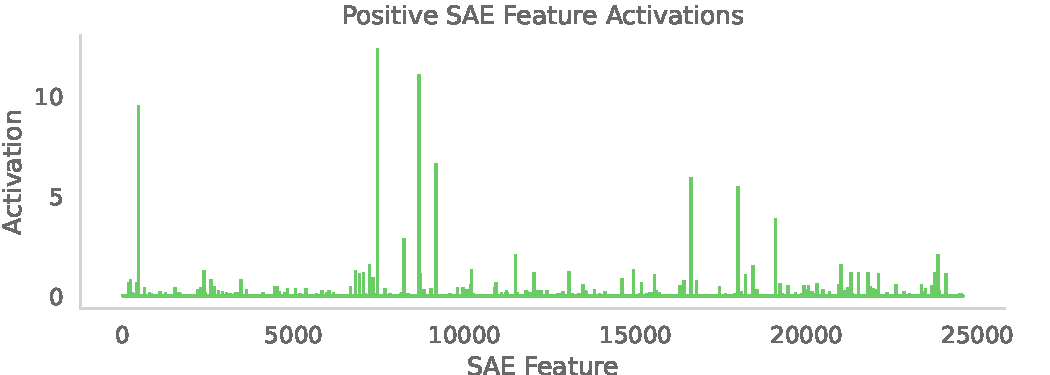
\includegraphics[width=\textwidth]{figures/positive_sae_acts.pdf}
    \caption{
        The average SAE feature activation on the last token across all the positive examples for a specific dataset.
        Note that the lines are thicker than the space on the x axis so that they are visible, in reality the average feature activation is sparser than it appears.
    }
    \label{fig:pos-sae}
\end{figure}

To evaluate how well the model steers the models internal representation recall the representation of an SAE activation in \cref{fig:sae-acts}.
A similar activation is presented in \cref{fig:pos-sae} except the figure presents \emph{an average} of all SAE activations for the positive examples.
A successful model would result in the models internal representation matching these concepts and therefore activating the same SAE features.
Therefore, the first metric calculates the proportion of the positive SAE features (those visualised in \cref{fig:pos-sae}) that the adaptor activates (e.g. those in \cref{fig:sae-acts}).\footnote{The phrase ``the adaptor activates'' means the SAE feature activations of the model when the adaptor is applied.}

\begin{figure}
    \centering
    \captionsetup{width=.9\textwidth}
    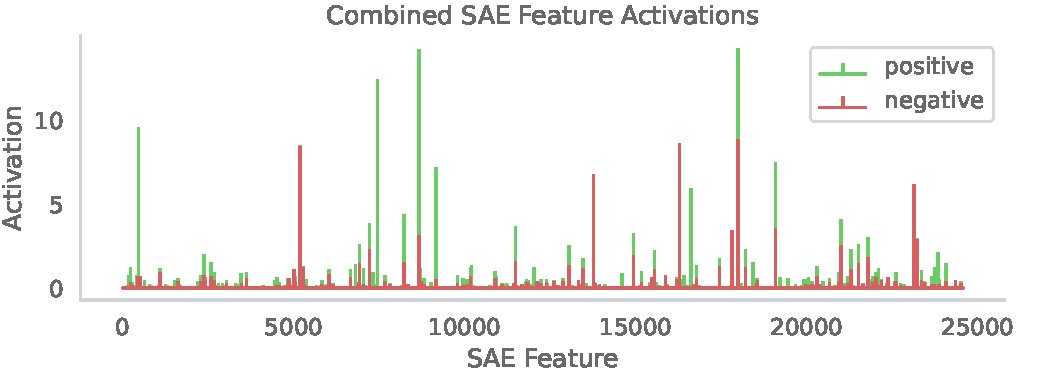
\includegraphics[width=\textwidth]{figures/combined_sae_acts.pdf}
    \caption{
        The combined average SAE feature activation on the last token across all examples for a specific dataset.
        Note that the lines are thicker than the space on the x axis so that they are visible, in reality the average feature activation is sparser than it appears.
    }
    \label{fig:comb-sae}
\end{figure}

It is important to ensure the model only affects the concepts present in the prompt and that which is being steered.
\cref{fig:comb-sae} shows the combined SAE feature activations for both the negative and positive examples.
There is a lot of overlap, relating to features that are activated by both examples (the context of the prompt), and some differences (the features specific to the positive and negative examples).
When steering the adaptor is likely to activate some or all of these features.
However, the adaptor should not activate the unactivated features as these are not correlated to either the prompt context or the steered concept.
The second metric captures this by calculating the proportion of this unactivated SAE features that the adaptor activates.

To calculate semantic similarity the model output is embedded into a vector space where distance represents semantic similarity.
This is achieved using Distilbert \citep{distilbert} which embeds text into vectors that preserve the semantics of the input text.
The cosine similarity between these embedded vectors represents how close in representation space the two phrases are and therefore how semantically similar the two phrases are.
This provides a metric for the semantic similarity of the models generated text and the target text.
The similarity of the prompt and the completion is used in its entirety to provide better context for the semantic similarity.

Each metric on its own is useful but can be prone to biases that the other metrics highlight.
A more complete picture of how the adaptors performed is achieved by analysing all three metrics together.

Finally, though this project aims to quantitatively analyse the performance of different adaptors on natural language it is important to see the generated completions.
In all three metrics it is possible for the adaptor to arbitrarily increase the quantitative value resulting in nonsense sentences.
This motivates the use of qualitative analysis alongside the quantitative analysis.
A selection of generated sentences across the adaptors, hyperparameters, and datasets is presented and analysed qualitatively.
Together with the quantitative analysis this provides verification of the adaptors performance whilst also providing an opportunity to evaluate the proposed metrics effectiveness.

\subsection{Hyperparameters}

Affine methods are agnostic to the dimension of the activations and so their hyperparameters should remain the same as {\scshape Steering Clear} \cref{sec:steering-clear}.
The hyperparameters are therefore $\lambda \in \{1, 2, 3, 5\}$ for CAA and $\lambda \in \{1, 2, 3, 5, 10\}$ for ACE.

The low-rank methods do, indirectly, rely on the dimension of the activations as they project the activations into a lower dimensional space.
Assuming that the optimal rank of the low-rank adaptor is linked to the dimension of the activations, and is not affected by superposition \cref{sec:sae}, an increase in activation dimension is expected to result in an increase in optimal rank.
In {\scshape Steering Clear} the activation dimension is 256 with corresponding hyperparameter values $\{1, 2, 3, 5, 10, 20\}$.
In the case of GPT-2 \cite{gpt-2} the activation dimension is 756, triple 256, therefore the hyperparameter values $\{3, 5, 10, 20, 30, 60\}$ are used.
